

% ARCHIVOS DE DATOS Y SUS DIFERENCIAS
  %\section{Características de los datos}

% RESULTADOS PARA ANISOTROPÍAS EN RA PARA LOS ICRC
  \section{Anisotropías en ascensión recta en los archivos del ICRC 2017 y ICRC 2019}

% ---> 8 EeV 
    \subsection{Eventos por encima de 8 EeV }

% ------> CARACTERISTICAS
     % \subsubsection{Características de los datos analizados}

% ------> ICRC 2017
      \subsubsection{Resultados para los datos del ICRC 2017}

      Para este apartado analicé el archivo de datos de la tesis de doctorado de Oscar Taborda, solamente los eventos 6T5. El rango de tiempo en el cual hice  el análisis es entre 1072969615 y 1472688000 ( 2004-01-01 15:06:55 y 2016-11-01 0:00:00 )

      Sabemos que para energía mayores de 8 EeV, aparece el dipolo en sidérea.

      En las Fig.\,\ref{fig:8EeV_sin_peso_ICRC2017_raw} y \ref{fig:8EeV_sin_peso_ICRC2017_cor} se muestra la amplitud del primer armónico sin considerar el peso de los hexágonos. Está figura es compatible con la Fig. 5.7.b, página 90 de la tesis de Taborda.

        \begin{figure}[H]
        
          \begin{subfigure}[b]{\textwidth}
          \centering
            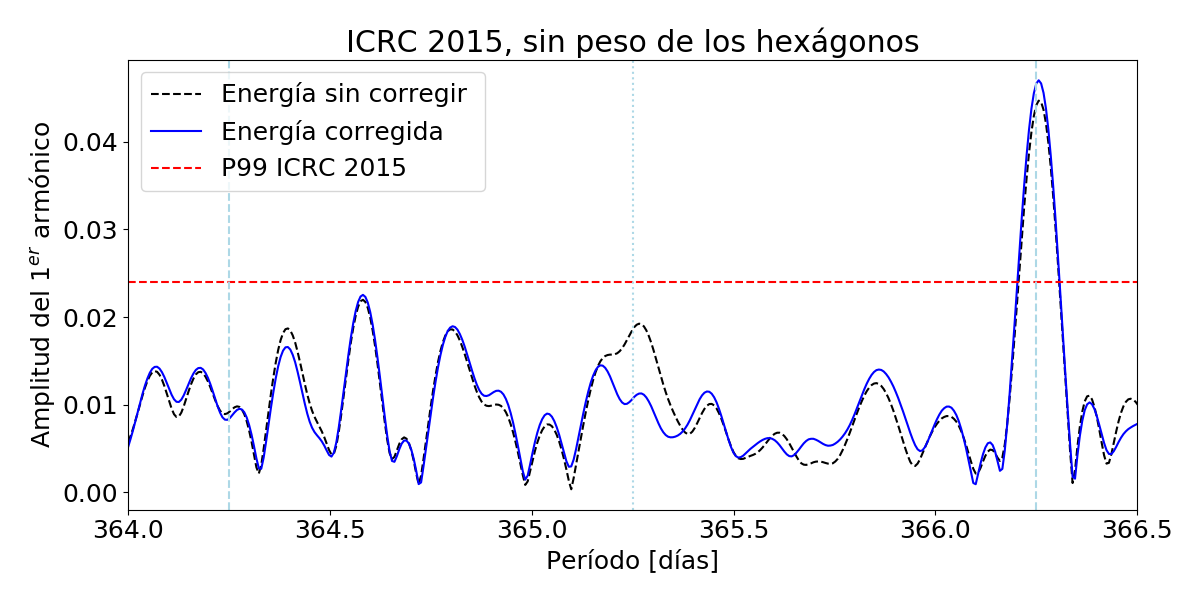
\includegraphics[width=\textwidth]{../0_Introduccion/ICRC/ICRC2017_Ecor_Eraw.png}
            \caption{Sin peso de la cantidad de tanques activos. }  \label{fig:8EeV_sin_peso_ICRC2017_raw}
          \end{subfigure}%
        
          \begin{subfigure}[b]{\textwidth}
          \centering
            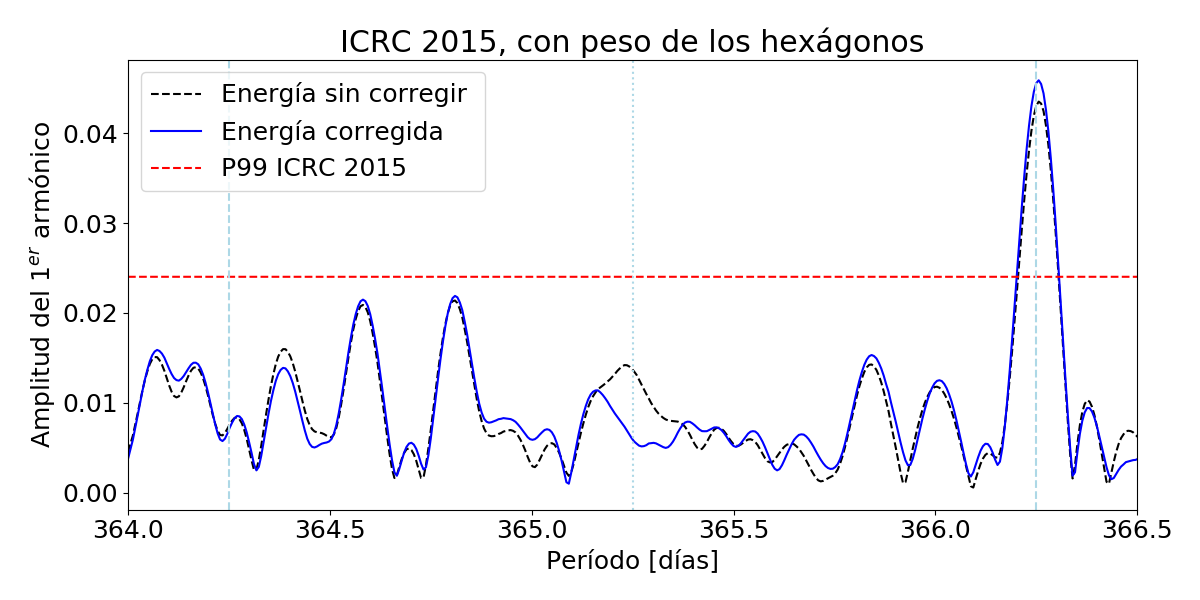
\includegraphics[width=\textwidth]{../0_Introduccion/ICRC/ICRC2017_Ecor_Eraw_hex.png}
            \caption{Con peso de la cantidad de tanques activos. }  \label{fig:8EeV_sin_peso_ICRC2017_cor}
          \end{subfigure}
          \caption{Primer armónico en ascensión recta de los datos del ICRC 2017}
        \end{figure}

      Con esto podemos decir que el código para la anisotropía funciona para el caso donde no se considera los hexágonos. No tengo un referencia para comparar las anisotropías con el peso de los hexágonos, solamente el valor del pico del dipolo.

% ------> ICRC 2019
      \subsubsection{Resultados para los datos del ICRC 2019}
      
      Este es el conjunto de archivos donde se hicieron modificaciones como el uso de una nueva reconstrucción y la corrección del clima. Usé solamente los eventos 6T5. El rango de tiempo en el cual hice  el análisis es entre 1072969615 y 1535789456 ( 2004-01-01 15:06:55 y   2018-09-01 08:10:56)

      \begin{figure}[H]
        \centering
        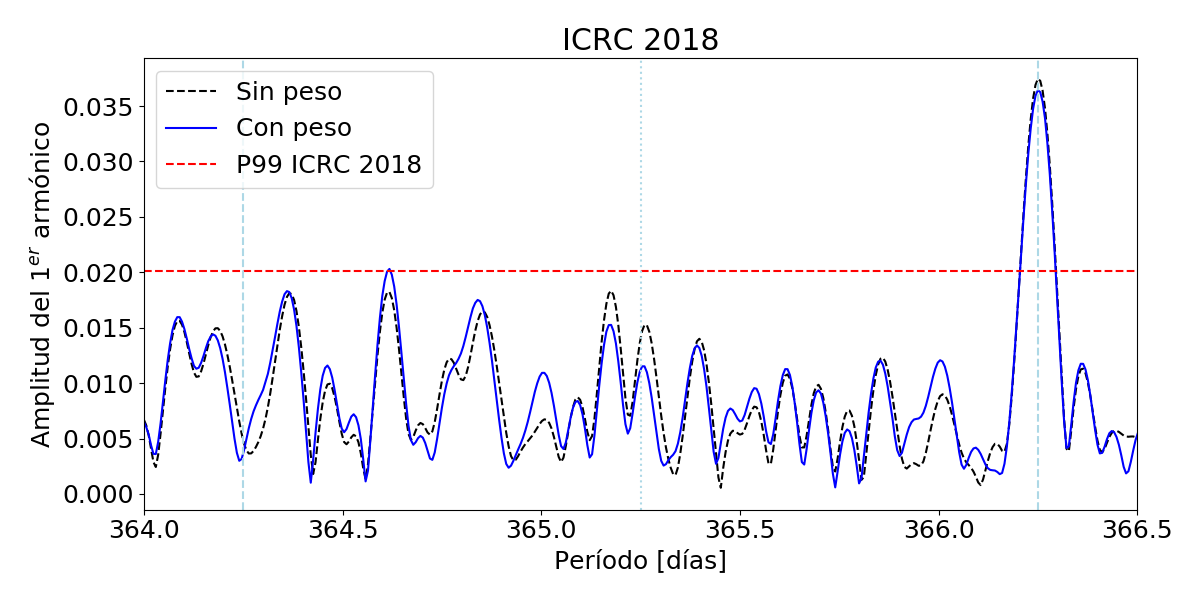
\includegraphics[width=\textwidth]{../0_Introduccion/ICRC/ICRC2019_Eraw_Eraw_hex.png}
        \caption{Primer armónico en ascensión recta de los datos del ICRC 2019.} \label{fig:8EeV_con_peso_ICRC2019}
      \end{figure}


      
% RESULTADOS PARA ANISOTROPÍAS EN RA PARA ALL TRIGGERS
  \section{Anisotropías en ascensión recta en los archivos con todos los disparos}
% ---> CARACTERISTICAS
    \subsection{Características de los archivos de datos analizados}

      Tenemos que tener en cuenta el archivo de datos de todos los disparos es entre los años 2013 y 2019, por lo que no podemos comparar los análisis de anisotropía con el conjunto  de datos del ICRC 2019 completo. Por lo que para compararlos, voy a hacer el análisis de ambos conjuntos de datos en el mismo rango de tiempo. Voy a hacer esto para poder comparar lo que sale.       Este rango donde se está comparando entre archivo empieza en  $utc_i = 1372699409 $.

    %CARACTERISTICAS GENERALES DE AMBOS SET DE DATOS.

      A continuación se presentan las características de los archivos estudiados, sin ningún filtro de energía, sin acotar por tiempo. 

      \begin{table}[H]
      \centering
        \begin{tabular}{c|c|c|c}
        \textbf{Archivo} & \text{Eventos} & UTC inicial &  UTC final  \\ \hline
        2020       & 13 739 351   &  1372680068 &  1577879983 \\
        2019       &  8 463 063   &  1372680068 &  1496318388 \\
        2017       &  8 592 302   &  1372680068 &  1498521517 \\
          \end{tabular}
      \end{table}
      
      Puede verse que el Archivo de 2020 tiene más eventos, y además de tener un rango de tiempo mayor que el archivo del 2017 y 2019. Los archivos 2017 y 2019  tienen $7\,072\,964$ eventos coincidentes y los archivos 2017 y 2020 tienen $6\,902\,21$ A continuación se compara la diferencia de energía y la calibración entre estos eventos.

    %COMPARANDO DELTA E ENTRE LOS DOS ARCHIVOS
      En las  Figs.\,\ref{fig:deltaE} y \ref{fig:histograma} se muestra la diferencia entre el valor de energía entre eventos coincidentes entre los archivos 2017 y 2020. Puede apreciarse que la diferencia no esta centrada 0 y no aparenta tener una modulación del clima. Por lo tanto la diferencia se debe a una reconstrucción distinta de los eventos.

          \begin{figure}[H]
            \begin{subfigure}[b]{0.5\textwidth}
              \centering
              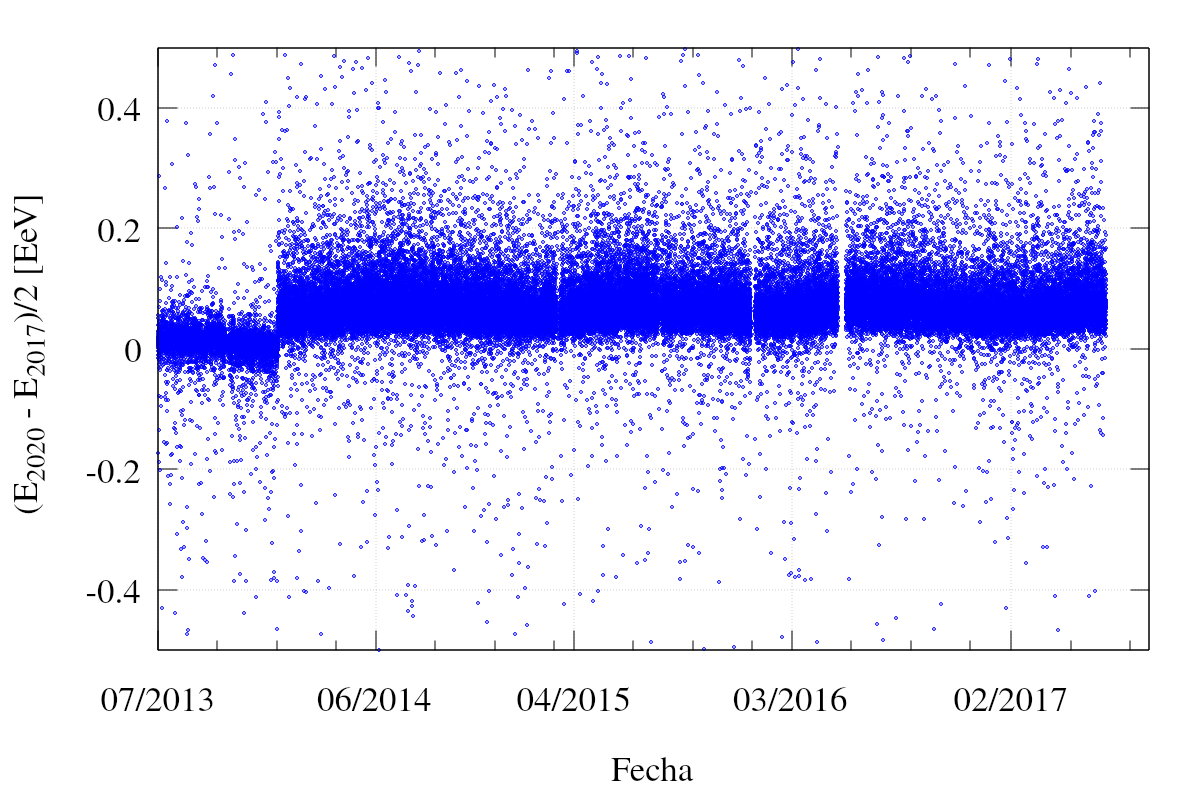
\includegraphics[width=\textwidth]{../0_Introduccion/comparacion_deltaE.png}
              \caption{Diferencia entre las energías} \label{fig:deltaE}
            \end{subfigure}%
            \begin{subfigure}[b]{0.5\textwidth}
              \centering
              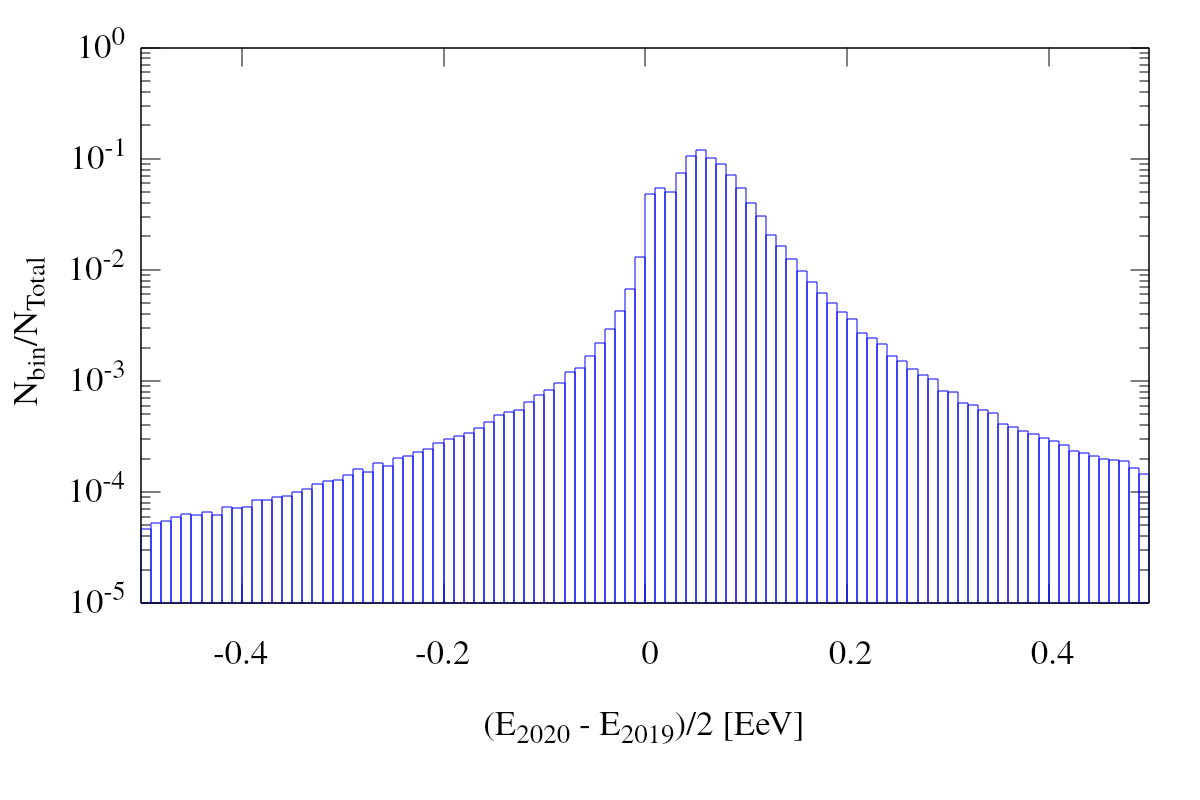
\includegraphics[width=0.8\textwidth]{../0_Introduccion/histograma_deltaE.png}
              \caption{Histograma de las diferencias}   \label{fig:histograma}
            \end{subfigure}
            \caption{Diferencia entre las energías del archivo de 2017 y el archivo del 2019}
          \end{figure}

    %COMPARANDO LA CURVA DE CALIBRACIÓN ENTRE LOS DOS ARCHIVOS
      Puede verse en la Fig.\,\ref{fig:calibracionE} que la curva de calibración entre ambos archivos es distinta, ya que la coordenada al origen como la pendiente es difieren entre para ambos archivos. Esto implica que los valores A y B de la curva $E=A\times (S_{38})^B$ son distintos para ambos conjunto de datos, ¿en qué afectaría? en primer lugar en el valor de la energía, segundo en análisis que dependan del estos parámetros como el análisis de la modulación del clima.

        \begin{figure}[H]
          \centering
          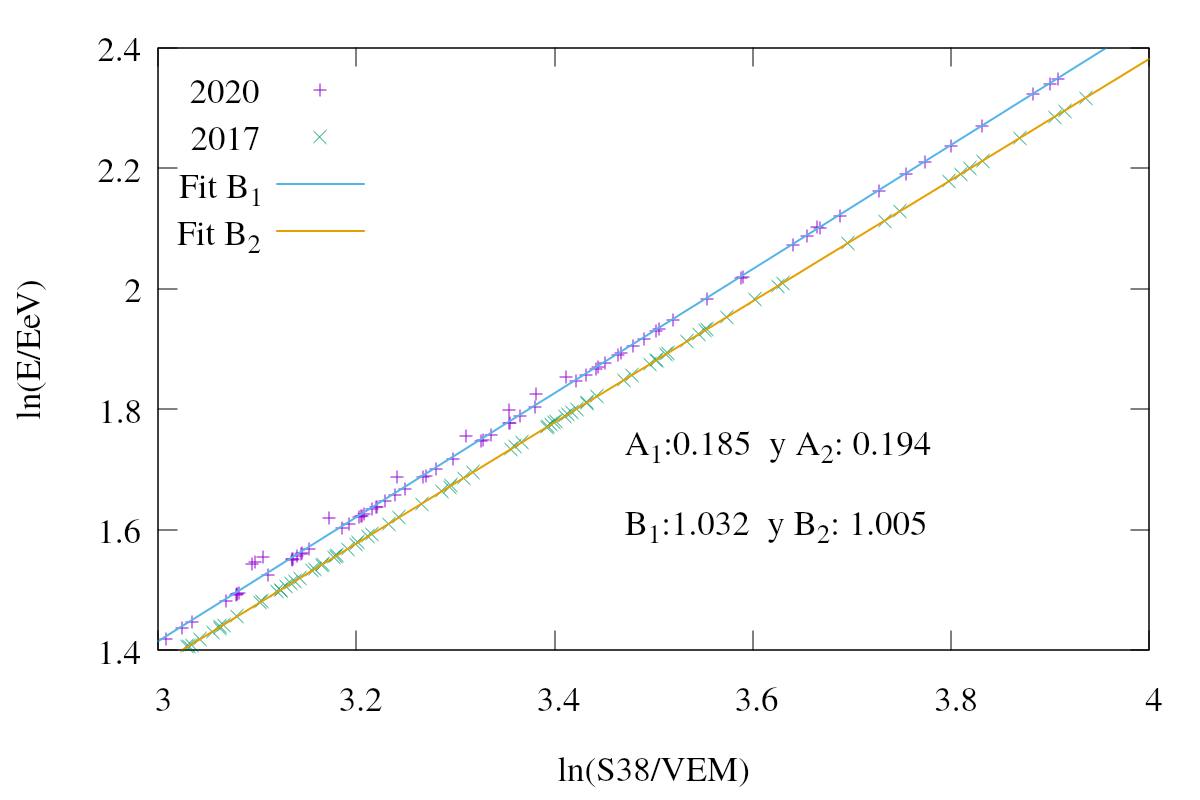
\includegraphics[width=0.65\textwidth]{../0_Introduccion/comparacion_reconstruccion.png}
          \caption{Calibración de las energías del archivo de 2017 y el archivo del 2019}
          \label{fig:calibracionE}
        \end{figure}

% % ---> 1 EeV 
%     \subsection{Eventos por encima de 1 EeV }
% % ------> CARACTERISTICAS
%       \subsubsection{Características de los datos analizados}

%       Comparando las cantidad de eventos por encima de 1 EeV para cada conjunto de datos

%         \begin{table}[H]
%           \centering
%             \begin{tabular}{c|c|c|c}
%             \textbf{Archivo} & \text{Eventos}   & UTC inicial &  UTC final  \\ \hline
%             2020       & 1\,515\,872    & 1372680308  & 1577879886 \\
%             %2019      & 647\, 656    & 1372699410  & 1496267276 \\
%             2017       & 635\, 353    & 1372680308  & 1496275090 \\
%             \end{tabular}
%         \end{table}

% {\bf hasta acá está verificado}
% ------> ALL TRIGGERS 2017
      % \subsubsection{Resultados del archivo de 2017}

      %   \begin{figure}[H]
      %     \centering
      %     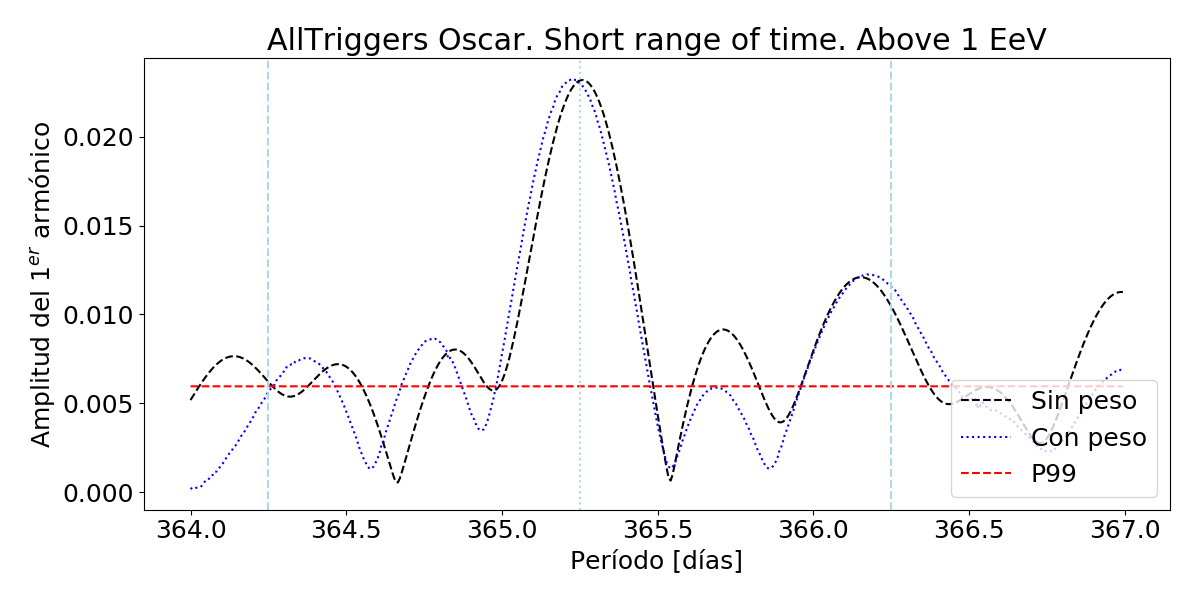
\includegraphics[width=0.95\textwidth]{../0_Introduccion/AllTriggers/AllTriggers_2017_Short_range_Above_1_EeV.png}
      %   \end{figure}
      % En el gráfico de todos los disparos para el archivo de 2017, se ve que hay una modulación anual importante. Es de esperarse ya que la correción del clima aun no fue implementada para este conjuntos de datos.

      % Comentario: {\sl Para el análisis en frecuencias, no hace ruido el hecho que la línea del P99 esté tan bajo, siendo que solo depende de la cantidad de eventos, }


% ------> ALL TRIGGERS 2019
    %\subsubsection{Resultados del archivo del 2020}

    %{\bf Esta sección no fue actualizada aún}
    % \begin{figure}[H]
    %   \centering
    %   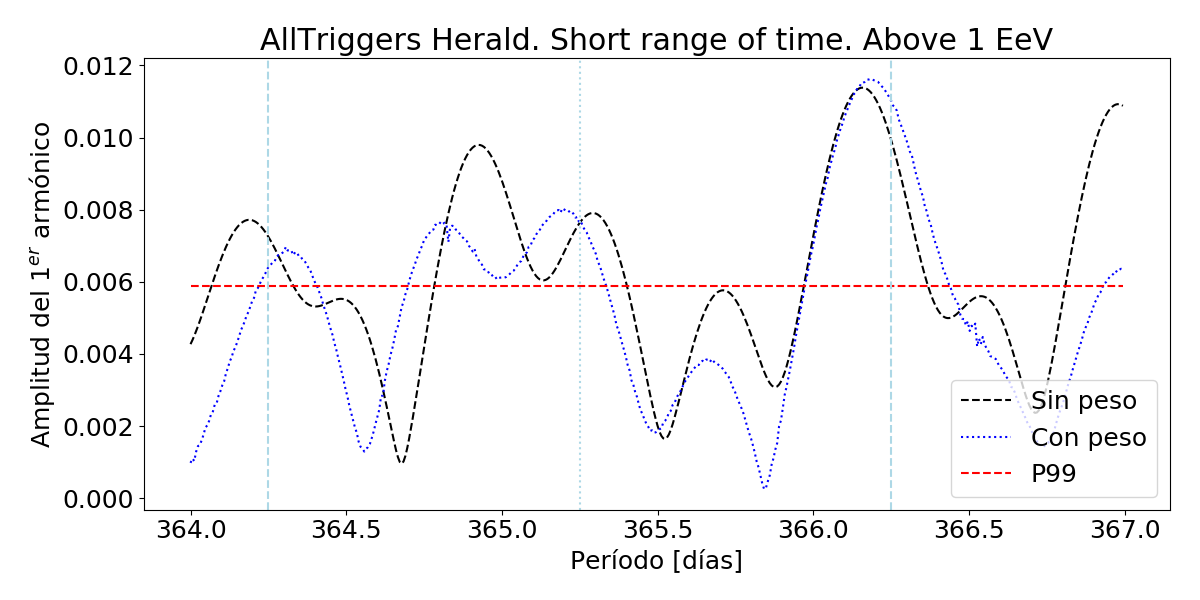
\includegraphics[width=0.95\textwidth]{../0_Introduccion/AllTriggers/AllTriggers_2019_Short_range_Above_1_EeV.png}
    % \end{figure}

% --> WEATHER STUFF
